\section{}

\begin{figure}[H]
	\centering
	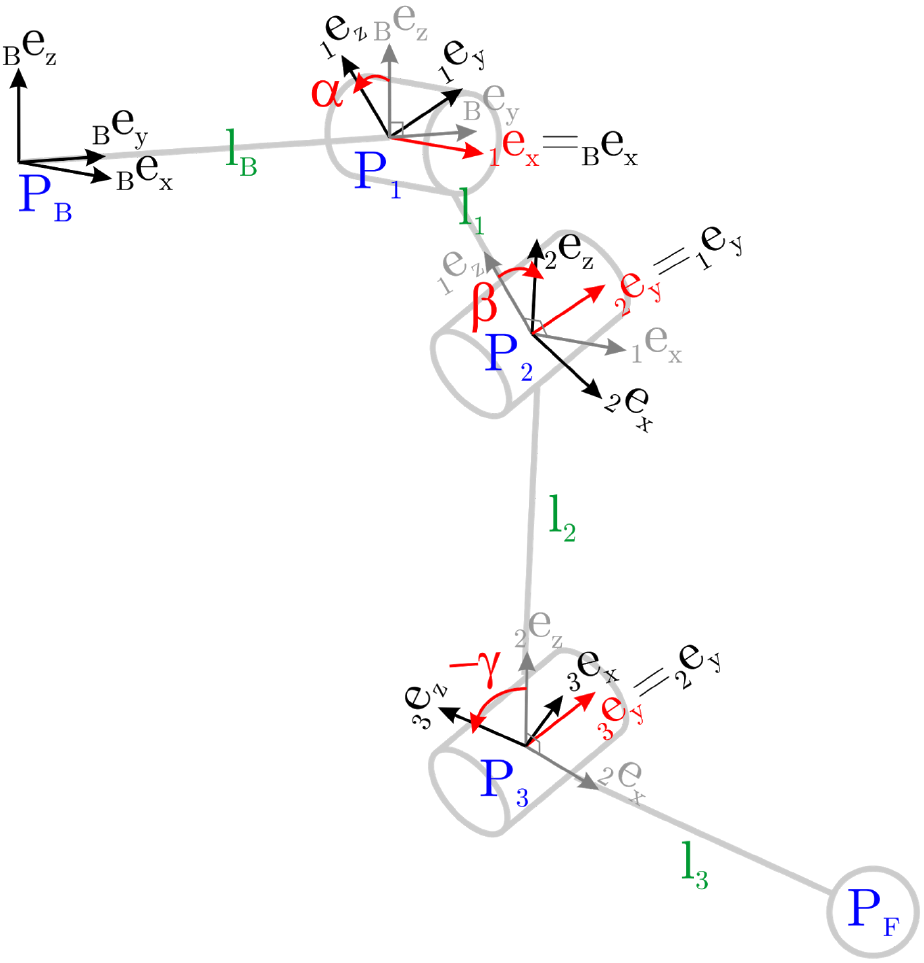
\includegraphics[width=0.5\linewidth]{img/robot_leg}
	\caption{Sistemas de coordenadas da perna robótica.}
	\label{fig:robot_leg}
\end{figure}

Uma vez dados os sistemas de coordenadas da perna robótica, exibidos na \autoref{fig:robot_leg}, é possível observar que o \textit{frame} \{$P_1$\} apresenta rotação em torno do eixo $x$, o \textit{frame} \{$P_2$\} em torno do eixo $y$, assim como o \textit{frame} \{$P_3$\}. Considerando o vetor de coordenadas generalizadas, $\+q = [\alpha \ \beta \ \gamma]^T$, sendo $\alpha, \ \beta $ e $\gamma$ respectivamente os ângulos de rotação dos sistemas de coordenadas \{$P_1$\}, \{$P_2$\} e \{$P_3$\}.

Com isso, têm-se que a rotação entre os sistemas de coordenadas da base e da junta 1 é dado pela matriz \eqref{eq:R_B1}, a rotação entre o \textit{frame} \{$P_1$\} e o \textit{frame} \{$P_2$\} é dada por \eqref{eq:R_12} e a rotação entre o sistema de coordenadas da junta 2 e o sistema da junta 3 é dado pela matriz \eqref{eq:R_23}.

\begin{equation}\label{eq:R_B1}
	\+R_{B1} = \begin{bmatrix}
		1 & 0          & 0 \\
		0 & \cos(\alpha) & -\sin(\alpha) \\
		0 & \sin(\alpha) & \cos(\alpha)
	\end{bmatrix}
\end{equation}

\begin{equation}\label{eq:R_12}
	\+R_{12} = \begin{bmatrix}
		\cos(\beta)  & 0  & \sin(\beta) \\
		0          & 1  & 0         \\
		-\sin(\beta) & 0  & \cos(\beta)
	\end{bmatrix}
\end{equation}

\begin{equation}\label{eq:R_23}
	\+R_{23} = \begin{bmatrix}
		\cos(\gamma) & 0 & \sin(\gamma) \\
		0            & 1 & 0            \\
		-\sin(\gamma)& 0 & \cos(\gamma)
	\end{bmatrix}
\end{equation}






\section{}

Os sistemas de coordenadas \{$P_B$\},  \{$P_1$\}, \{$P_2$\} , \{$P_3$\} e \{$P_F$\} da perna robótica estão posicionados entre eles em distâncias $l_B$, $l_1$, $l_2$, $l_3$ e $l_F$, respectivamente. Considerando todas essas distâncias iguais e unitárias, obtêm-se os vetores de translação entre os referenciais mostrados em \eqref{eq:r_B1_inB}, \eqref{eq:r_12_in1}, \eqref{eq:r_23_in2} e \eqref{eq:r_3F_in3}.

\begin{equation}\label{eq:r_B1_inB}
	_B \+r_{B1} = \begin{bmatrix} 0 & 1 & 0 \end{bmatrix}^T;
\end{equation}


\begin{equation}\label{eq:r_12_in1}
	_1 \+r_{12} =  \begin{bmatrix} 0 & 0 & -1 \end{bmatrix}^T;
\end{equation}


\begin{equation}\label{eq:r_23_in2}
	_2 \+r_{23} = \begin{bmatrix} 0 & 0 & -1 \end{bmatrix}^T;
\end{equation}


\begin{equation}\label{eq:r_3F_in3}
	_3 \+r_{3F} = \begin{bmatrix} 0 & 0 & -1 \end{bmatrix}^T;
\end{equation}

Permitindo a transformação entre os sistemas de coordenada, incluindo rotação e translação em uma só operação, a utilização de transformações homogêneas se faz interessante, sendo a mesma enunciada em \eqref{eq:H}.

\begin{equation}
	\+H = \begin{bmatrix}
		&	\+R_{[3\times 3]} & & \+{r}_{[3\times 1]} \\
		0 & 0 & 0 & 1
	\end{bmatrix}_{[4\times 4]}
	\label{eq:H}
\end{equation}

Dessa forma, a transformação homogênea entre o \textit{frame}  \{$P_B$\} e  \{$P_1$\} é dada por \eqref{eq:H_B1}, entre \{$P_1$\} e  \{$P_2$\} é dada por \eqref{eq:H_12},  entre \{$P_2$\} e  \{$P_3$\} é dada por \eqref{eq:H_23} e  entre \{$P_3$\} e  \{$P_F$\} é dada por \eqref{eq:H_3F}, 

\begin{equation}\label{eq:H_B1}
	_B \+H_{1} = \begin{bmatrix}
		1 & 0            & 0              & 0\\
		0 & \cos(\alpha) & -\sin(\alpha)  & 1\\
		0 & \sin(\alpha) & \cos(\alpha)   & 0 \\
		0 & 0 & 0                         & 1
	\end{bmatrix}
\end{equation}


\begin{equation}\label{eq:H_12}
	_1 \+H_{2} = \begin{bmatrix}
		\cos(\beta)  & 0  & \sin(\beta)  &  0 \\
		0          & 1  & 0                  &  0 \\
		-\sin(\beta) & 0  & \cos(\beta)      & -1  \\
		0 & 0 & 0 & 1
	\end{bmatrix}
\end{equation}


\begin{equation}\label{eq:H_23}
	_2 \+H_{3} = \begin{bmatrix}
		\cos(\gamma)  & 0  & \sin(\gamma)  &  0 \\
		0          & 1  & 0                  &  0 \\
		-\sin(\gamma) & 0  & \cos(\gamma)      & -1  \\
		0 & 0 & 0 & 1
	\end{bmatrix}
\end{equation}


\begin{equation}\label{eq:H_3F}
	_3 \+H_{F} = \begin{bmatrix}
		1 & 0  & 0      &  0 \\
		0 & 1  & 0      &  0 \\
		0 & 0  & 1      & -1  \\
		0 & 0  & 0      & 1
	\end{bmatrix}
\end{equation}

Para se obter a transformação homogênea entre \textit{frames} de um conjunto consecutivo de transformações de referencial, basta multiplicar as matrizes de transformação homogênea, como feito em \eqref{eq:HB3}, obtendo assim a transformação da base para a terceira junta da perna robótica.

\begin{equation}\label{eq:HB3}
	_B \+H_3 \ = \ _B \+H_1 \  _1 \+H_2  \ _2 \+H_3 = \begin{bmatrix}
[            \text{c}(\beta + \gamma) &          0 &             \text{s}(\beta + \gamma) &                            -\text{s}(\beta) \\
 \text{s}(\beta + \gamma)\text{s}(\alpha) & \text{c}(\alpha) & -\text{c}(\beta + \gamma)\text{s}(\alpha) & \text{s}(\alpha) + \text{c}(\beta)\text{s}(\alpha) + 1 \\
-\text{s}(\beta + \gamma)\text{c}(\alpha) & \text{s}(\alpha) &  \text{c}(\beta + \gamma)\text{c}(\alpha) &           -\text{c}(\alpha)(\text{c}(\beta) + 1) \\
                            0 &          0 &                             0 &                                     1 
	\end{bmatrix}
\end{equation}

\begin{align}\label{eq:HBF}
	_B \+H_F \ &= \ _B \+H_1 \  _1 \+H_2  \ _2 \+H_3  \ _3 \+H_F  \\ &= \begin{bmatrix}
            \text{c}(\beta + \gamma) &          0 &             \text{s}(\beta + \gamma) &                                                                           - \text{s}(\beta + \gamma) - \text{s}(\beta) \\
 \text{s}(\beta + \gamma)\text{s}(\alpha) & \text{c}(\alpha) & -\text{c}(\beta + \gamma)\text{s}(\alpha) & \text{s}(\alpha)[1 +\text{c}(\beta) + \text{c}(\beta)\text{c}(\gamma) - \text{s}(\beta)\text{s}(\gamma)] + 1 \\
-\text{s}(\beta + \gamma)\text{c}(\alpha) & \text{s}(\alpha) &  \text{c}(\beta + \gamma)\text{c}(\alpha) &                                                           -\text{c}(\alpha)[\text{c}(\beta + \gamma) + \text{c}(\beta) + 1] \\
                            0 &          0 &                             0 &                                                                                                         1
	\end{bmatrix} \nonumber
\end{align}

Por meio da transformação de referencial entre o \textit{frame} da base e da ferramenta, \eqref{eq:HBF}, é possível expressar o vetor da base para a ferramentam, pré-multiplicando o vetor da origem da base ($_B\+r_{BB} = [0 \ 0 \ 0]^T_B$) pela transformação homogênea em questão.

\begin{equation}\label{eq:r_BF_inB}
	_B \+r_{BF} = \ _B\+H_F \ _B\+r_{BB} = \begin{bmatrix} - \sin(\beta + \gamma) - \sin(\beta) \\ \sin(\alpha)[\cos(\beta + \gamma) + \cos(\beta) + 1] + 1  \\ -\cos(\alpha)[\cos(\beta + \gamma) + cos(\beta) + 1] \end{bmatrix}
\end{equation}





\section{}

\begin{gather}\label{eq:J_BF_inB}
	_B \+J_{BF} = \frac{\partial _B \+r_{BF}}{\partial \+q} = \begin{bmatrix}
		\frac{\partial _B \+r_{BF}}{\partial q_1} & \frac{\partial_B \+r_{BF}}{\partial q_2} & \frac{\partial _B \+r_{BF}}{\partial q_3}\end{bmatrix} = \begin{bmatrix}
		\frac{\partial _B r_{xBF}}{\partial q_1} & \frac{\partial_B r_{xBF}}{\partial q_2} & \frac{\partial _B r_{xBF}}{\partial q_3} \\
		\frac{\partial _B r_{yBF}}{\partial q_1} & \frac{\partial_B r_{yBF}}{\partial q_2} & \frac{\partial _B r_{yBF}}{\partial q_3} \\
		\frac{\partial _B r_{zBF}}{\partial q_1} & \frac{\partial_B r_{zBF}}{\partial q_2} & \frac{\partial _B r_{zBF}}{\partial q_3} 
	\end{bmatrix} \\
	_B \+J_{BF} = \begin{bmatrix}
	0	& -\text{c}(\beta + \gamma) - \text{c}(\beta)  & -\text{c}(\beta + \gamma) \\
	\text{c}(\alpha)[\text{c}(\beta + \gamma) + \text{c}(\beta) + 1]	& \text{s}(\alpha)[-\text{s}(\beta + \gamma) -\text{s}(\beta)] & -\text{s}(\alpha)\text{s}(\beta + \gamma) \\
	\text{s}(\alpha)[\text{c}(\beta + \gamma) + \text{c}(\beta) + 1]	&  \text{c}(\alpha)[\text{s}(\beta + \gamma) +\text{s}(\beta)] & \text{c}(\alpha)\text{s}(\beta + \gamma)
	\end{bmatrix}
\end{gather}

Onde $\text{s}(\cdot) = \sin(\cdot)$ e $\text{c}(\cdot) = \cos(\cdot)$.

Considerando uma posição inicial para a perna robótica, \eqref{eq:qi}, e uma velocidade para a ferramenta \eqref{eq:v}, obtém-se um jacobiano instantâneo igual a \eqref{eq:JBF}.

\begin{equation}\label{eq:qi}
	\+q_i = \begin{bmatrix}
		0^\circ & 60^\circ & -120^\circ
	\end{bmatrix}^T
\end{equation}

\begin{equation}\label{eq:v}
	\+v = \begin{bmatrix}
		0 & 0 & -1\end{bmatrix}^T \text{(m/s)}
\end{equation}

\begin{equation}\label{eq:JBF}
	\+J_{BF} = \begin{bmatrix}
		0 & -1 & -0,5 \\
		2 & 0 & 0 \\
		0 & 0 & 0,866
	\end{bmatrix}
\end{equation}

Com isso, uma vez que o jacobiano relaciona a velocidade no espaço cartesiano com a velocidade no espaço das juntas, $\+v = \+J\+{\Dot{q}}$, pode-se obter a velocidade instantânea das das juntas da perna robótica, $\text{d}\+q$, por meio de \eqref{eq:dq}, para a velocidade desejada do efetuador e a posição inicial das juntas.

\begin{equation}\label{eq:dq}
	\text{d}\+q = \+J_{BF}^+ \+v = \begin{bmatrix}0 \\ -0,5774 \\ 1,1547 	\end{bmatrix}
\end{equation}





\section{}

Para realizar o posicionamento do manipulador em um ponto desejado, deve-se fazer o uso da cinemática inversa, porém, sua obtenção de forma analítica é um procedimento por muitas vezes complexo e massante. Dessa forma, pode-se fazer o uso de métodos numéricos, como o de Newton, para convergir para a posição desejada do efetuador em $n$ passos, até que o erro $\zeta$ seja menor que o desejado.

\begin{equation}\label{eq:qi+}
	\+q^{i+1} = \+q^i + \+J^+ (\+r^{goal} - \+r^i)
\end{equation}

Por meio do Algoritmo~\ref{alg:qi+}, é feita a resolução da cinemática inversa de forma numérica, atualizando a posição da perna robótica a cada interação para acompanhamento da convergência do algoritmo.

\begin{algorithm}
	\caption{Cinemática inversa numérica}\label{alg:qi+}
	\begin{algorithmic}[1]
		\State $\zeta \gets 0.01$; \Comment Stop error
		\State $\+q^i \gets \+q^0$;
		
		\While{$ ||\+r^{goal} - \+r^i||_2 \ge \zeta$}\Comment{While solution does not converge...}
			
	 		\State $\+q^{i+1} \gets \+q^i + \text{pinv}(\+J(\+q^i))*(\+r^{goal} - \+r^i)$;
			
			\Call{UpdateRobotLegPosition}{ $\+q^{i+1}$};
			
			\State $\+q^i \gets \+q^{i+1}$;
			
		\EndWhile
		
		\State $\+q^{goal} \gets \+q^i$ \Comment{Generalized coordinates for the solution}
		
	\end{algorithmic}
\end{algorithm}

\begin{figure}[H]
	\centering
	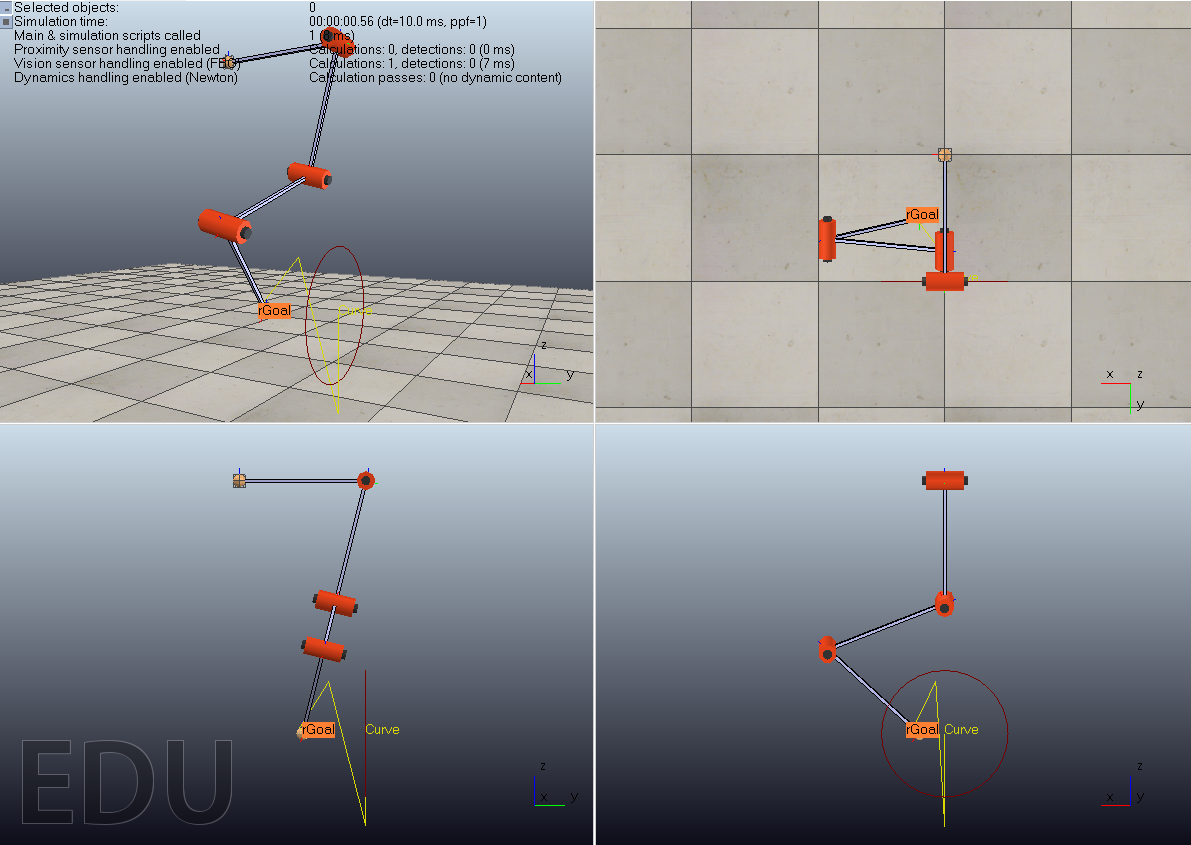
\includegraphics[width=0.75\linewidth]{img/ex4}
	\caption{Posicionamento da perna robótica em uma posição desejada por meio da cinemática inversa numérica.}
	\label{fig:ex4}
\end{figure}

A convergência se deu em três passos, como mostrado no \textit{log} abaixo.

\begin{verbatim}
i = 1 | rGoal = [0.200 0.500 -2.000]; r = [0.000 1.000 -2.732]; error = 0.478 
i = 2 | rGoal = [0.200 0.500 -2.000]; r = [0.071 0.706 -1.589]; error = 0.072 
i = 3 | rGoal = [0.200 0.500 -2.000]; r = [0.249 0.476 -1.953]; error = 0.003 
\end{verbatim}


\section{}

Uma vez dada os \textit{waypoints} da trajetória a ser seguida pela perna robótica, faz-se o uso novamente da relação \eqref{eq:dq} para obtenção da velocidade dos atuadores. Porém, dessa vez $\+v$ será dado com base no erro de posição entre o efetuador da perna robótica e o ponto da trajetória atual, multiplicado por um ganho proporcional, como em \eqref{eq:ev}.

\begin{equation}\label{eq:ev}
	\+v = K_p(\+r^{goal} - \+r^{i})
\end{equation}

Considerando um ganho proporcional igual $K_p = 10$, obteve-se um bom rastreio da trajetória, com um transitório consideravelmente curto, e boa convergência ao \textit{setpoint}, como pode ser visto nas Figuras~\ref{fig:Ex5_effector_position}~e~\ref{fig:Ex5_effector_position_3d}.

\begin{figure}[H]
	\centering
	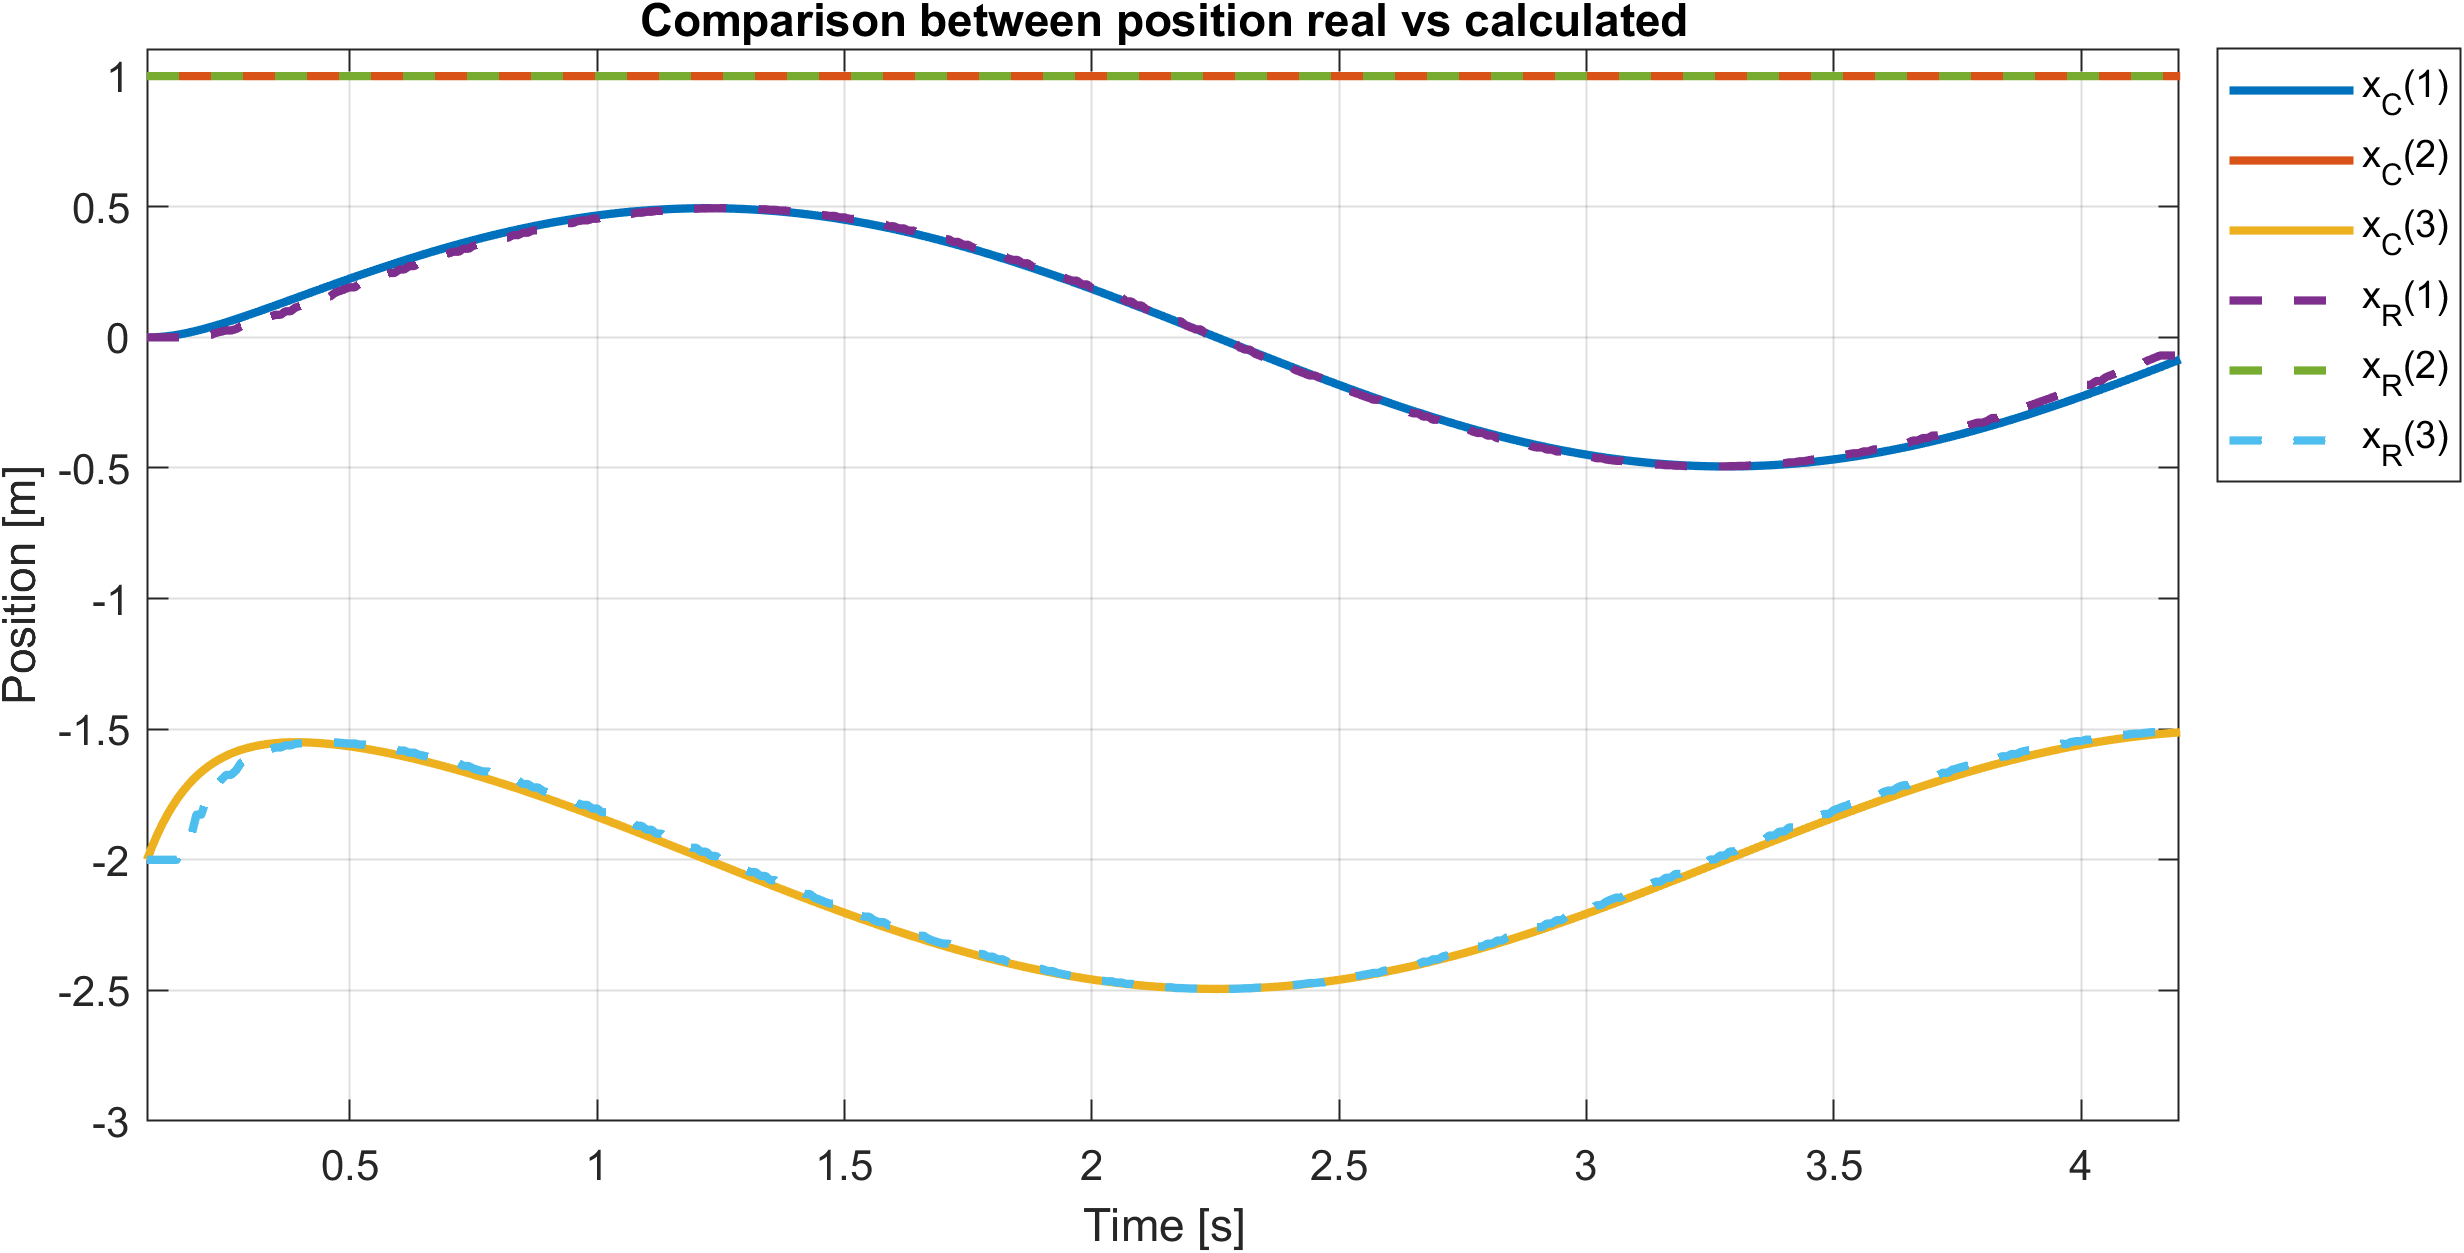
\includegraphics[width=0.75\linewidth]{img/Ex5_effector_position}
	\caption{Rastreio da posição do efetuador da perna robótica em $x$, $y$ e $z$.}
	\label{fig:Ex5_effector_position}
\end{figure}

\begin{figure}[H]
\centering
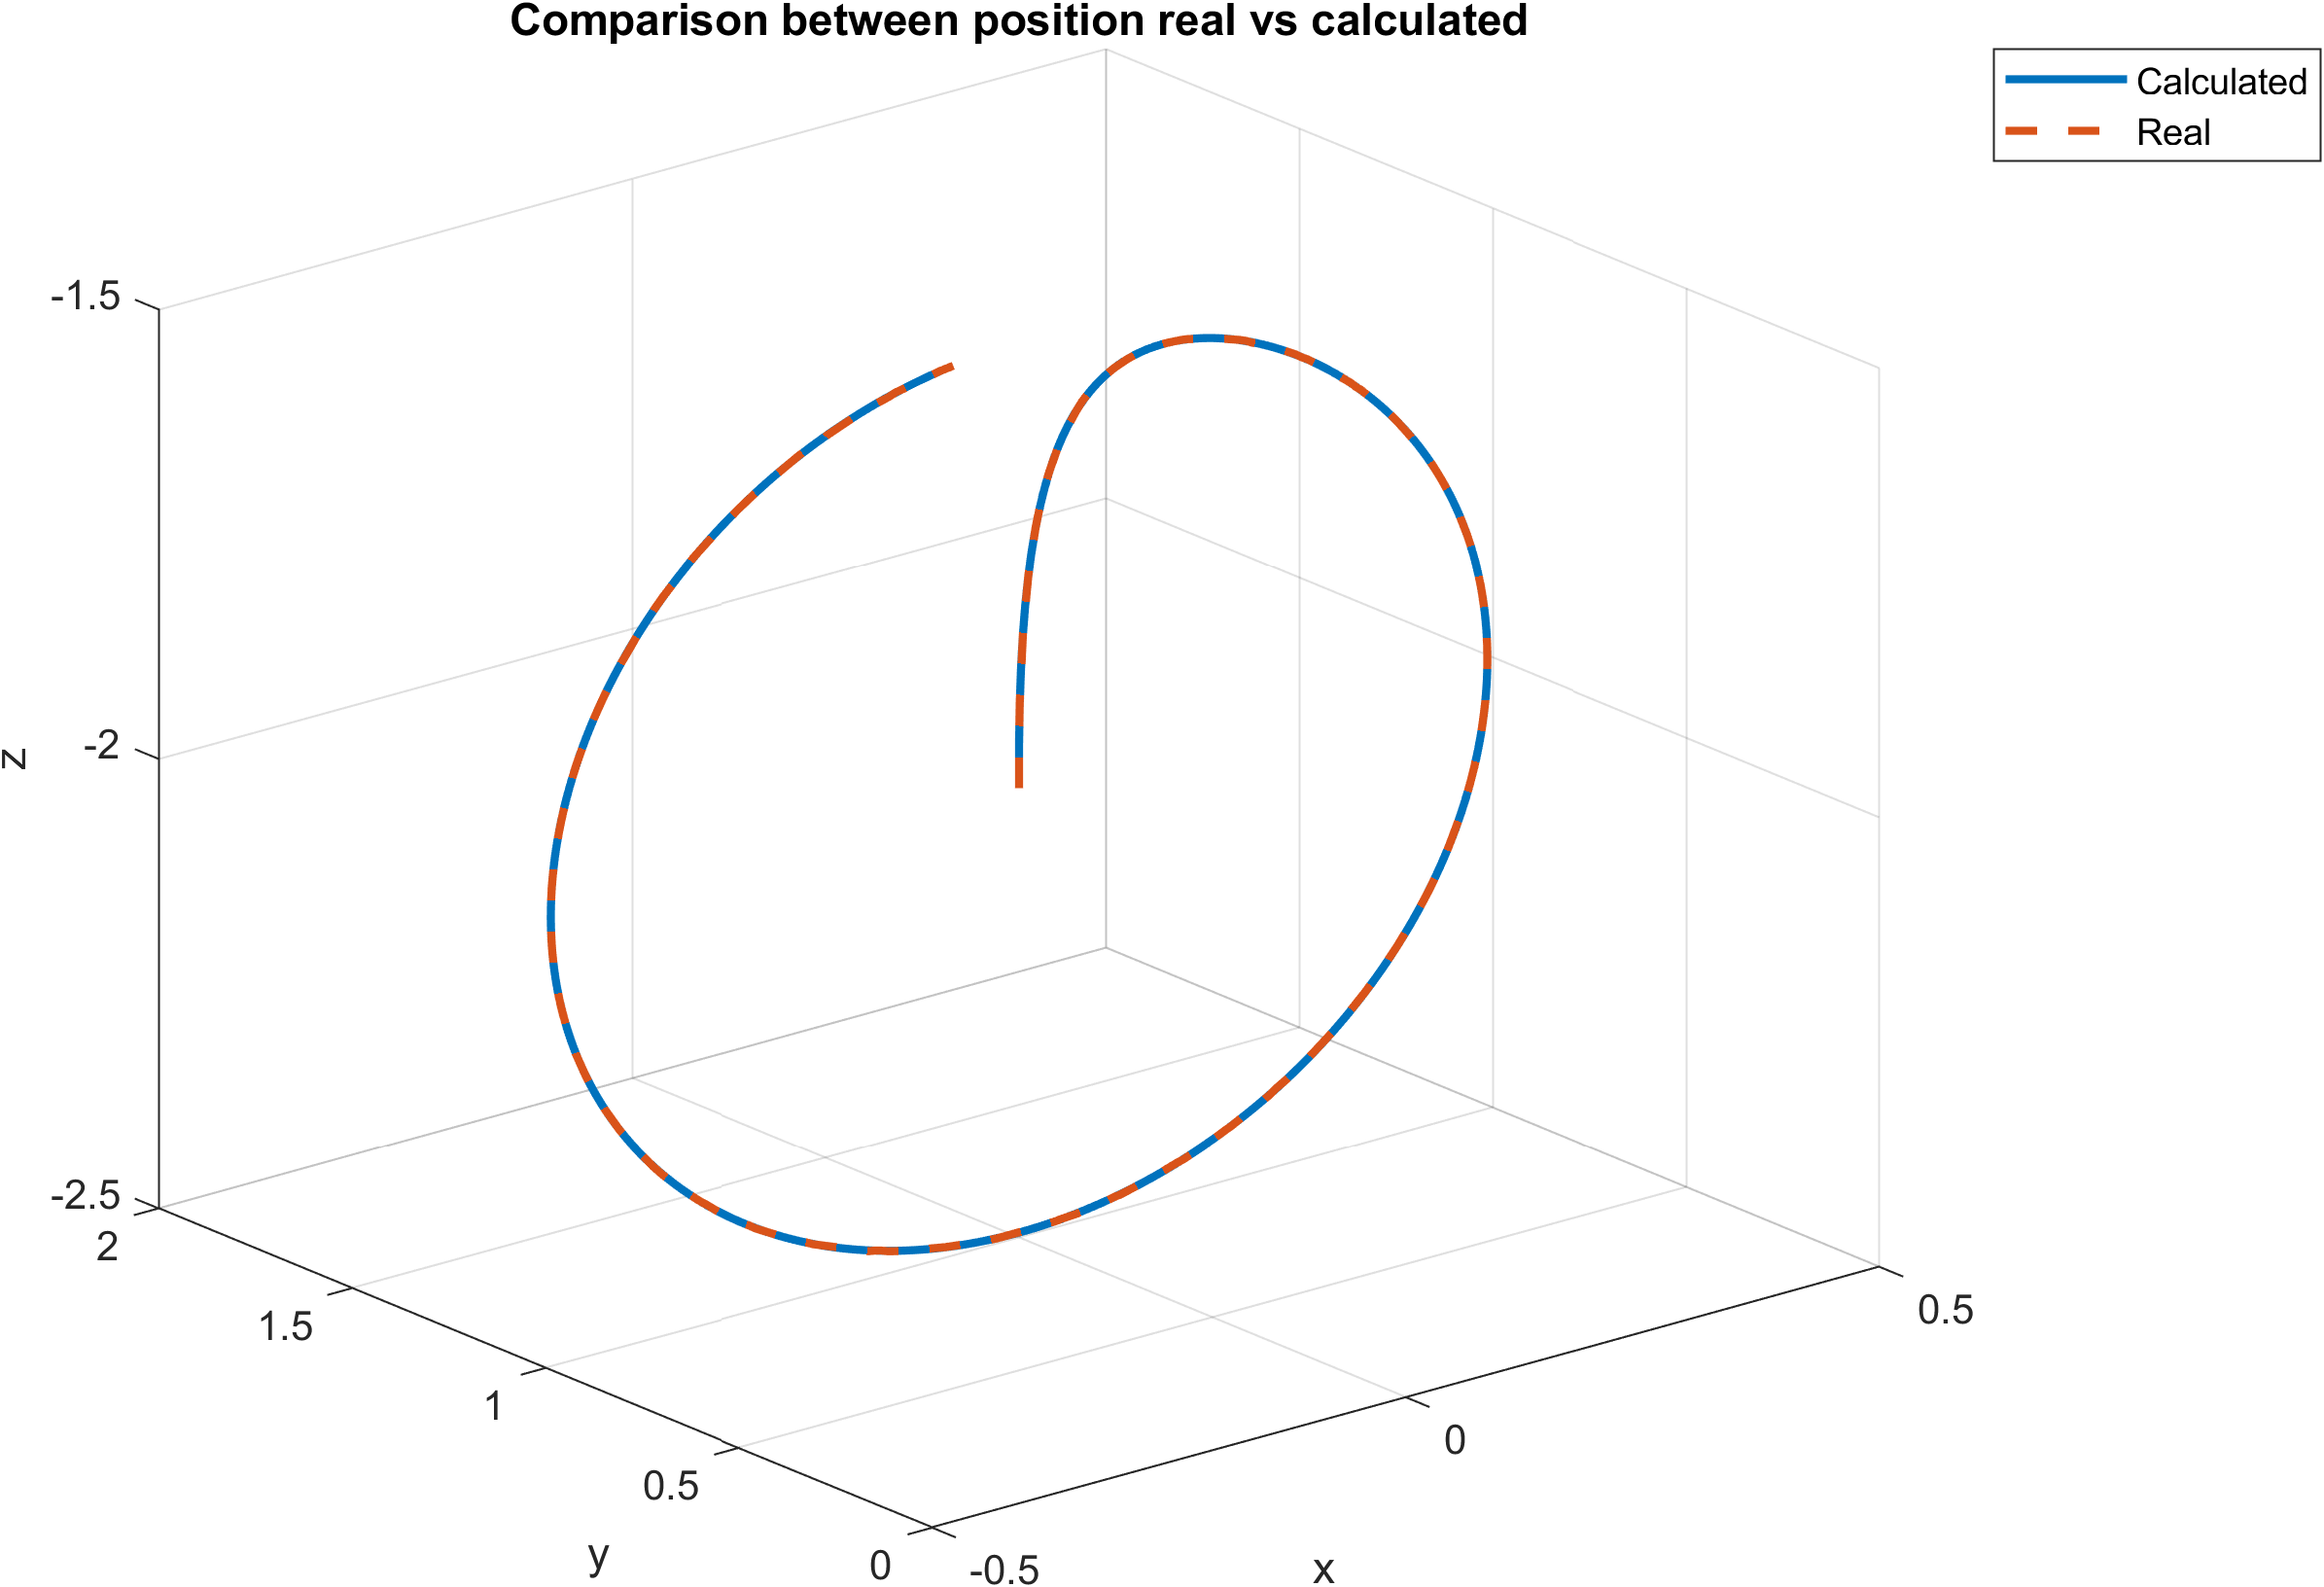
\includegraphics[width=0.75\linewidth]{img/Ex5_effector_position_3d}
\caption{Rastreio da posição do efetuador da perna robótica no espaço.}
\label{fig:Ex5_effector_position_3d}
\end{figure}

Por fim, é possível observar na Figura~\ref{fig:ex5} a trajetória realizada pela perna robótica partindo da posição inicial no centro do círculo.

\begin{figure}[H]
	\centering
	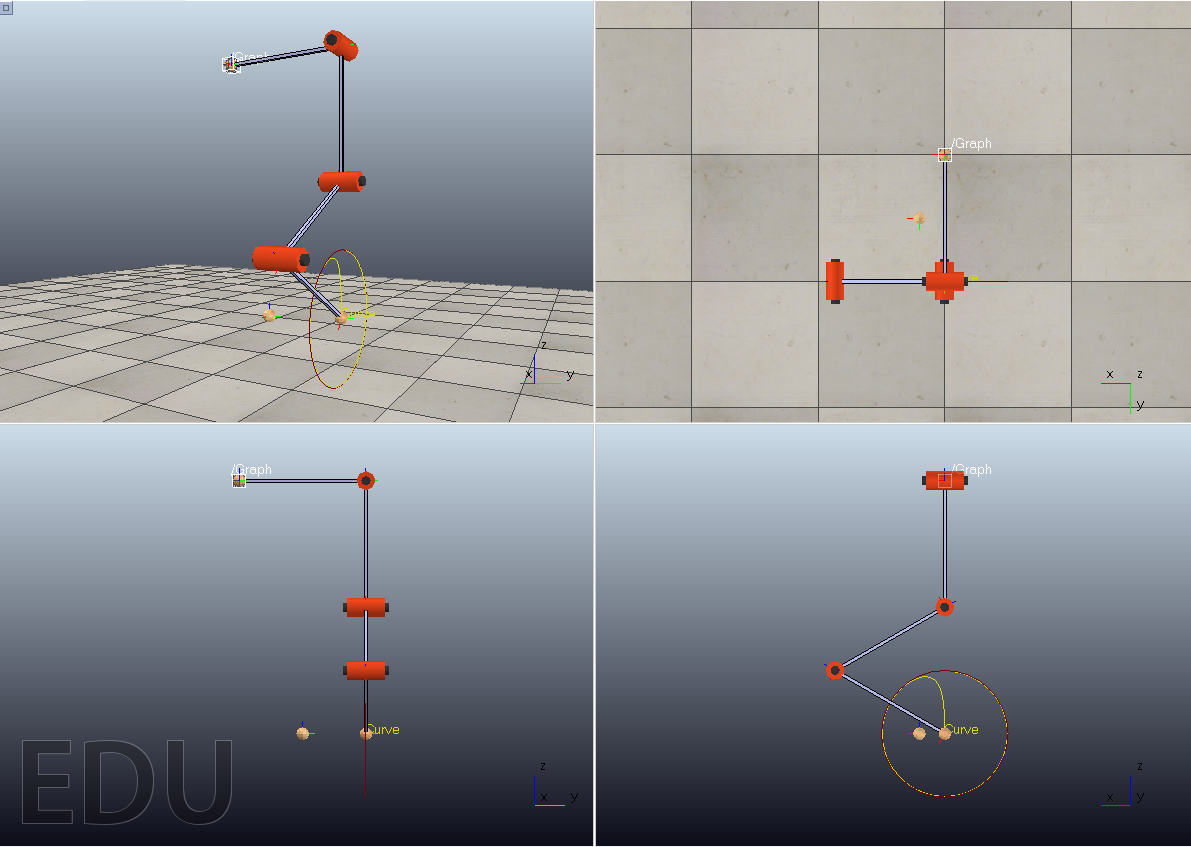
\includegraphics[width=0.75\linewidth]{img/ex5}
	\caption{Trajetória realizada pela perna robótica.}
	\label{fig:ex5}
\end{figure}

